%
% Tugas Akhir S1 Teknik Elektro
%
% Muhammad Adeel Mahdi Suviyanto (1102183191)
% S1 Teknik Elektro
% Fakultas Teknik Elektro
% Telkom University
%
% Dokumen ini dibuat sesuai dengan kaidah format penulisan Tugas Akhir di Telkom University,
% dengan standar sitasi IEEE.


% Klasifikasi dokumen sebagai report, single column
\documentclass[12pt, a4paper, oneside]{book}

% Load file konfigurasi
%
% Konfigurasi LaTeX Tugas Akhir
%
% Muhammad Adeel Mahdi Suviyanto (1102183191)
% S1 Teknik Elektro
% Fakultas Teknik Elektro
% Telkom University
%
%
%

%Data buku
%Judul laporan
\newcommand{\judul}{Pengembangan Algoritma Komunikasi Antar-Unmanned Aerial Vehicle Berbasis \textit{PainlessMesh} Pada Mikrokontroler ESP32}
%Judul laporan, kapital
\newcommand{\JUDUL}{PENGEMBANGAN ALGORITMA KOMUNIKASI ANTAR-UNMANNED AERIAL VEHICLE BERBASIS \textit{PAINLESSMESH} PADA MIKROKONTROLER ESP32}

%Thesis title
\newcommand{\juduleng}{Development of an Inter-Unmanned Aerial Vehicle Communications Algorithm based on PainlessMesh using an ESP32 Microcontroller}
%Thesis title, in caps
\newcommand{\JUDULENG}{DEVELOPMENT OF AN INTER-UNMANNED AERIAL VEHICLE COMMUNICATIONS ALGORITHM BASED ON PAINLESSMESH USING AN ESP32 MICROCONTROLLER}

%Tahun publikasi
\newcommand{\tahun}{2022}
%Tanggal pengesahan
\newcommand{\tanggalpengesahan}{x Juli 2022}

%Data penulis
%Nama penulis
\newcommand{\penulis}{Muhammad Adeel Mahdi Suviyanto}
%Nama penulis, kapital
\newcommand{\PENULIS}{MUHAMMAD ADEEL MAHDI SUVIYANTO}
%NIM
\newcommand{\nim}{1102183191}
%Email penulis
\newcommand{\email}{adeelsuviyanto@gmail.com}
%Program Studi
\newcommand{\prodi}{S1 Teknik Elektro}
%Gelar yang akan diperoleh
\newcommand{\gelar}{Sarjana Teknik}
%Program kuliah
\newcommand{\program}{Teknik Elektro Universitas Telkom}
%Fakultas
\newcommand{\fakultas}{Fakultas Teknik Elektro}
%Fakultas, kapital
\newcommand{\FAKULTAS}{FAKULTAS TEKNIK ELEKTRO}
%Universitas
\newcommand{\universitas}{Telkom University}

%Data Pembimbing
%Pembimbing 1
\newcommand{\pembimbingsatu}{Dr. Eng. Willy Anugrah Cahyadi, S.T, M.T}
\newcommand{\pembimbingdua}{Ir. Uke Kurniawan Usman, M.T}

%
% Document packages!
%
% Atur sesuai kebutuhan, masih berbasis pada format Proposal Tugas Akhir
%
\usepackage{array}
\usepackage[indonesian]{babel}
\usepackage{amsmath} %Penulisan notasi matematika
\usepackage{amsfonts}
\usepackage{amssymb}
\usepackage{graphicx} %Memasukkan gambar ke laporan
\usepackage{fontenc}
\usepackage{pslatex} %Times New Roman
\usepackage{hyperref}
\usepackage[a4paper, lmargin=4cm, rmargin=3cm, tmargin=3cm, bmargin=3cm]{geometry}
\usepackage[backend=biber, style=ieee, language=english]{biblatex}
\usepackage{csquotes}
\usepackage{fancyhdr} %Header and footer
\usepackage{longtable}
\usepackage{caption} %Caption gambar
\usepackage{setspace}
	\onehalfspacing %Set line spacing ke 1.5
\usepackage[ConnyRevised]{fncychap}
\usepackage{titlesec}
\usepackage{tocloft}
\usepackage{enumitem}
\usepackage{indentfirst}
\usepackage{float}
\usepackage{adjustbox}
\usepackage{multirow}
%
% Chapter style setup
%
\titleformat{\chapter}[display]{\bfseries\large\centering}{BAB \thechapter}{1pt}{}[]
\titlespacing*{\chapter}{0pt}{-50pt}{1.5pt}
%setup section style
\titleformat{\section}[hang]{\bfseries\normalsize}{\thesection \ }{1pt}{}[]
\titlespacing*{\section}{0pt}{0pt}{1.5pt}
\titleformat{\subsection}[hang]{\bfseries\normalsize}{\thesubsection \ }{1pt}{}[]
\titleformat{\subsubsection}[hang]{\bfseries\normalsize}{\thesubsubsection \ }{1pt}{}[]

%set biblatex file
\addbibresource{./src/ta.bib}
\addbibresource{./src/references.bib}
\addbibresource{./assets/zoteroexport.bib}

%disable numbering for front matter
\newenvironment{unnumbered}
{\global\chardef\keeplevel=\value{secnumdepth}%
	\setcounter{secnumdepth}{-1}}
{\setcounter{secnumdepth}{\keeplevel}}

%dotted line for TOC
\renewcommand{\cftpartleader}{\cftdotfill{\cftdotsep}} % for parts
\renewcommand{\cftchapleader}{\cftdotfill{\cftdotsep}} % for chapters

% Load file BibLaTeX
\addbibresource{./src/references.bib,./src/ta.bib,./assets/zoteroexport.bib }

% Start dari dokumen
\begin{document}
	
% Cover
\begin{titlepage}
	\begin{center}
	\thispagestyle{empty}
	\Large
	\textbf{\JUDUL}
	\bigskip
	
	\textbf{\textit{\JUDULENG}}
	\bigskip
	
	\normalsize
	\textbf{TUGAS AKHIR}\\
	Disusun sebagai syarat mata kuliah Tugas Akhir\\
	Program Studi \prodi
	
	\bigskip
	Disusun oleh:\\
	\textbf{\PENULIS}\\
	\textbf{\nim}\\
	\bigskip
	\bigskip
	\bigskip
	
\includegraphics[scale=0.33]{./assets/logotelu.png}
	\vfill
	\Large
	\textbf{FAKULTAS TEKNIK ELEKTRO}\\
	\large
	\textbf{UNIVERSITAS TELKOM}\\
	\textbf{BANDUNG}\\
	\textbf{2022}
	\end{center} %akhir dari center, mulai dari sini pake subfile
\end{titlepage}

	

% Menyalakan penomoran halaman, angka romawi
\frontmatter
\pagestyle{myheadings}
\setcounter{page}{1}
	
% Halaman pengesahan
\addcontentsline{toc}{chapter}{LEMBAR PENGESAHAN}
\chapter*{LEMBAR PENGESAHAN} %Lembar Pengesahan sebagai Chapter


\begin{center} %2 halaman pertama all pake center
	\large
	\textbf{TUGAS AKHIR}
	\bigskip
	
	\Large
	\textbf{\JUDUL}
	\bigskip
	
	\textbf{\textit{\JUDULENG}}
	\bigskip
	\bigskip
	\bigskip
	
	\normalsize
	\textbf{Telah disetujui dan disahkan sebagai Buku Tugas Akhir}\\
	\textbf{Program Studi \prodi}\\
	\textbf{\fakultas}\\
	\textbf{\universitas}\\
	\bigskip
	\bigskip
	
	\textbf{Disusun oleh:}\\
	\textbf{\PENULIS}\\
	\textbf{\nim}\\
	\bigskip
	\bigskip
	
	\textbf{Bandung, x Juli 2021}\\
	\begin{tabular}{|p{6cm}|p{6cm}|}
		\hline
		Pembimbing 1 & Pembimbing 2 \\
		& \\
		& \\
		& \\
		Dr. Eng. Willy Anugrah Cahyadi, S.T, M.T. & Ir. Uke Kurniawan Usman,M.T. \\
		\hline
	\end{tabular}
\end{center}



% Halaman pernyataan orisinalitas
\chapter*{LEMBAR PERNYATAAN ORISINALITAS}
\bigskip

\begin{tabbing}
	\hspace{30mm}\=\hspace{5mm}\=\kill
	Nama \> : \> \penulis \\
	NIM \> : \> \nim \\
	Alamat \> : \> Taman Alfa Indah D4/11, Joglo, Kembangan, Jakarta Barat \\
	No Tlp/HP \> : \> 021 73443989 / 087777882699 \\
	Email \> : \> adeelsuviyanto@student.telkomuniversity.ac.id \\
\end{tabbing}
\bigskip

\noindent Menyatakan bahwa Tugas Akhir ini merupakan karya orisinal saya sendiri dengan judul:
\bigskip\\
\textbf{\judul} \\
\textbf{\textit{\juduleng}}
\bigskip\\
Atas pernyataan ini, saya siap menanggung risiko/sanksi yang dijatuhkan kepada saya apabila kemudian ditemukan adanya pelanggaran terhadap kejujuran akademik atau etika keilmuan dalam karya ini, atau ditemukan bukti yang menunjukkan ketidak aslian karya ini.\\
\bigskip\\



\begin{minipage}{0.3\textwidth}
	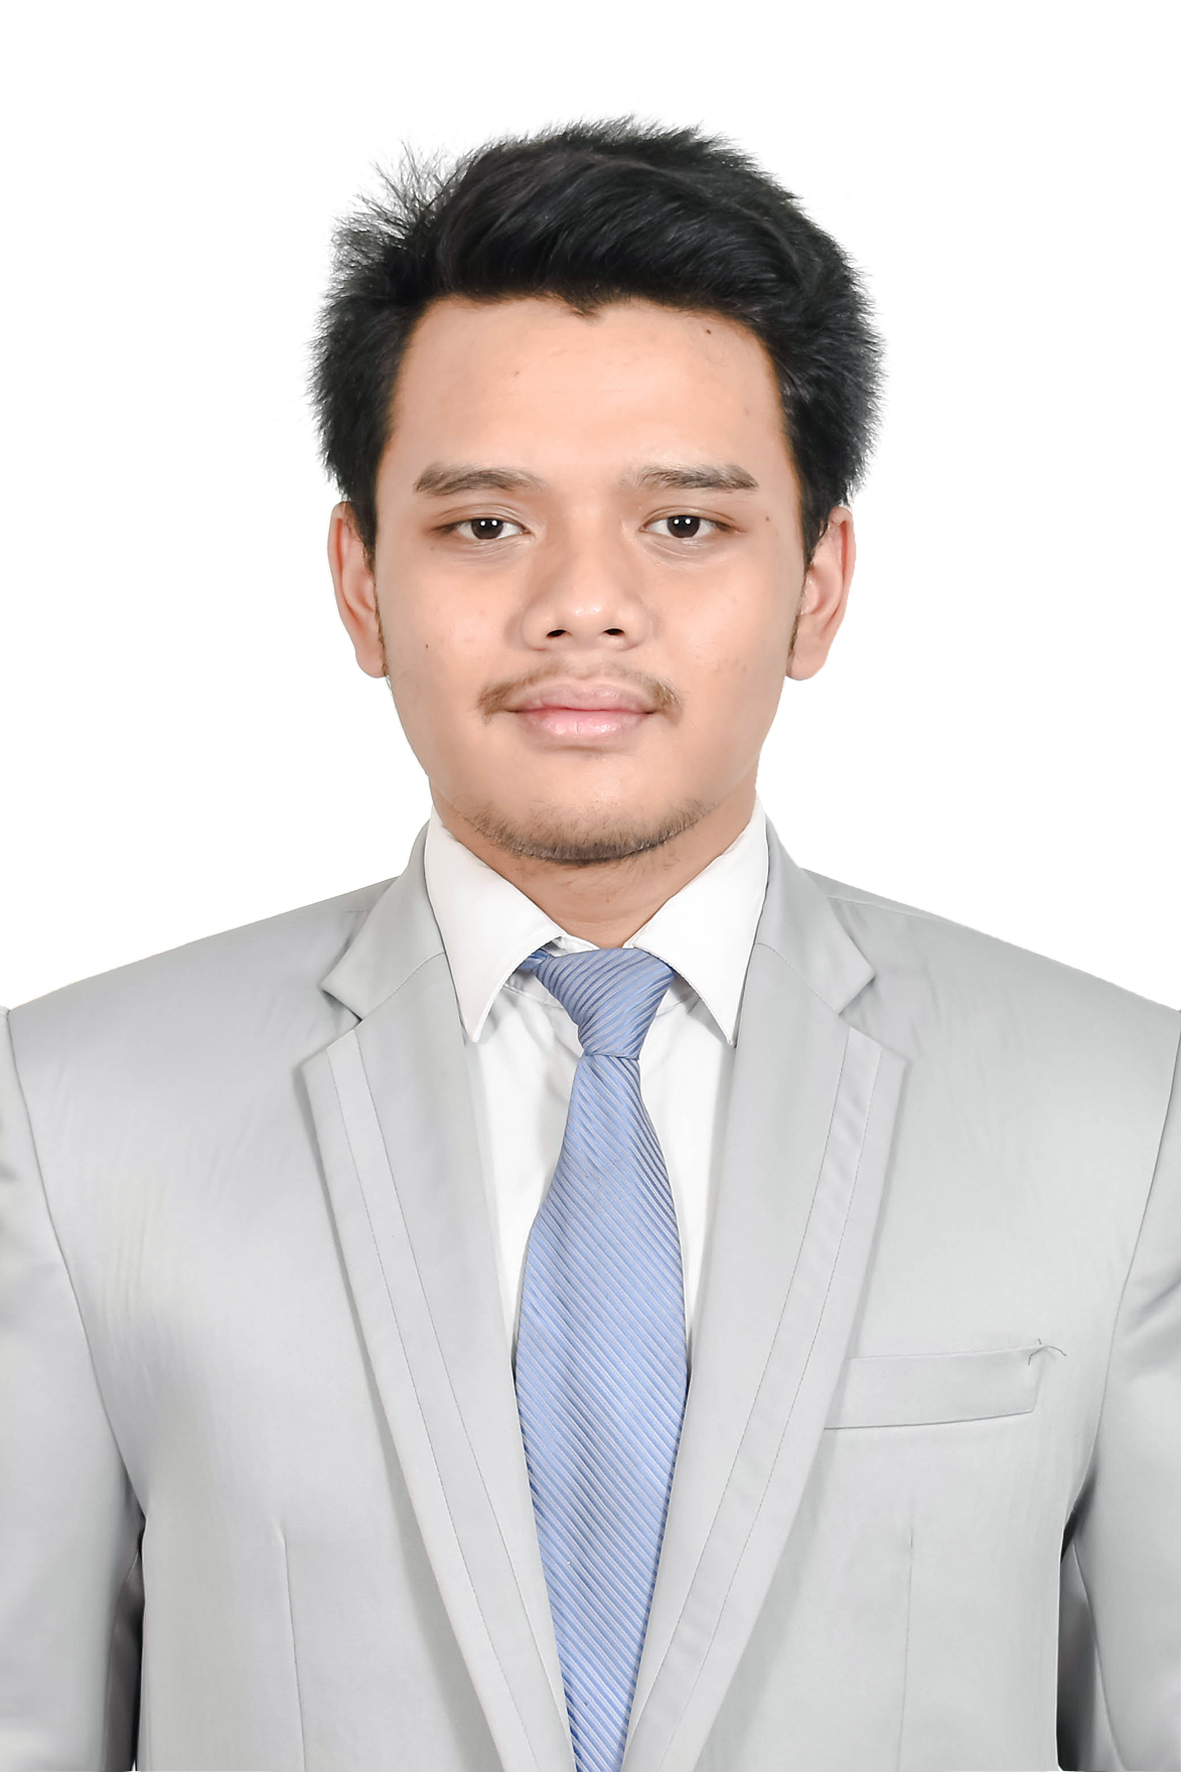
\includegraphics[scale=0.4] {./assets/PASFOTO}
\end{minipage}
\begin{minipage}{0.6\textwidth}\raggedleft
	Bandung, 25 Agustus 2022\\
	\vspace{1em}
	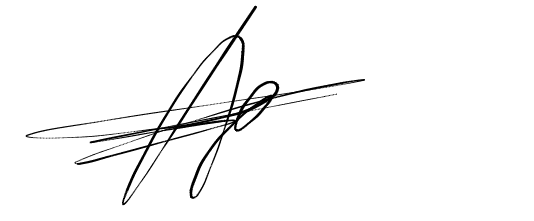
\includegraphics[scale=0.3]{./assets/signature}\\
	\vspace{1em}
	\penulis\\
	\nim
\end{minipage}

% Abstrak
\addcontentsline{toc}{chapter}{ABSTRAK}
\chapter*{ABSTRAK}

Salah satu faktor penentu kesuksesan dalam operasi \textit{Search and Rescue} (SAR) pada bencana alam adalah kecepatan dalam menemukan lokasi dan posisi korban serta pengiriman logistik bantuan penunjang hidup bagi korban tersebut. Penggunaan \textit{Unmanned Aerial Vehicle} dapat mendukung operasi SAR, dan untuk meningkatkan koordinasi antar UAV dalam sistem maka dikembangkan sebuah algoritma komunikasi antar-UAV. Model komunikasi yang dikembangkan berupa \textit{Flying Ad-hoc Network} (FANET), dan teknologi komunikasi yang dipilih berupa Wi-Fi menggunakan mikrokontroler ESP32 dan \textit{library} PainlessMesh. Kinerja jaringan diuji dari nilai \textit{throughput, packet loss,} dan \textit{round-trip delay}. Penelitian ini menghasilkan sebuah jaringan mesh dengan jarak antar node ESP32 hingga 50 meter, mampu mengirimkan data lokasi dari drone \textit{sender} ke drone \textit{receiver} dengan nilai \textit{packet loss} sebesar x persen, \textit{throughput} jaringan median sebesar x B/s, dan \textit{round-trip delay} median sebesar x ms. Analisis regresi linear menunjukkan korelasi antara \textit{throughput, round-trip delay,} dan \textit{packet loss} terhadap \textit{signal strength} antar node, dimana nilai \textit{signal strength} yang semakin mengecil menghasilkan kinerja jaringan yang menurun.

\vspace{2em}
\noindent \textbf{Kata kunci:} PainlessMesh, ESP32, \textit{Unmanned Aerial Vehicles}, \textit{Drone}, Komunikasi
% Abstract
\addcontentsline{toc}{chapter}{ABSTRACT}
\chapter*{ABSTRACT}

Placeholder text for Abstract.
% Kata Pengantar
\addcontentsline{toc}{chapter}{KATA PENGANTAR}
\chapter*{KATA PENGANTAR}

Placeholder text for Abstract.
% Ucapan Terima Kasih
\addcontentsline{toc}{chapter}{UCAPAN TERIMA KASIH}
\chapter*{UCAPAN TERIMA KASIH}

Placeholder text for Abstract.

%Menggunakan angka romawi dalam penomoran bab
\renewcommand{\thechapter}{\Roman{chapter}}
\renewcommand{\thesection}{\arabic{chapter}.\arabic{section}}
\renewcommand{\thefigure}{\arabic{chapter}.\arabic{figure}}
\renewcommand{\thetable}{\arabic{chapter}.\arabic{table}}
% Daftar isi
\addcontentsline{toc}{chapter}{DAFTAR ISI}
\chapter*{DAFTAR ISI}
\renewcommand*\contentsname{\vspace*{-3cm}}
\tableofcontents
% Daftar gambar
\addcontentsline{toc}{chapter}{DAFTAR GAMBAR}
\chapter*{DAFTAR GAMBAR}
\renewcommand*\listfigurename{\vspace*{-2cm}}
\listoffigures
% Daftar tabel
\addcontentsline{toc}{chapter}{DAFTAR TABEL}
\chapter*{DAFTAR TABEL}
\renewcommand*\listtablename{\vspace*{-2cm}}
\listoftables
% Daftar singkatan
\addcontentsline{toc}{chapter}{DAFTAR SINGKATAN}
\chapter*{DAFTAR SINGKATAN}


% Mulai bagian utama tugas akhir
\mainmatter
% Bab 1
\chapter{PENDAHULUAN}

\section{Latar Belakang Masalah}
Salah satu faktor penentu kesuksesan dalam operasi \textit{Search and Rescue} (SAR) pada bencana alam adalah kecepatan dalam menemukan lokasi dan posisi korban serta pengiriman logistik bantuan penunjang hidup bagi korban tersebut. Namun, kondisi daratan medan bencana alam yang sukar dilewati oleh tim penyelamat dapat menyebabkan lamanya kedua proses tersebut, menurunkan probabilitas keselamatan bagi korban \cite{syafitriAutonomousDisasterVictim2020}. Pada saat ini, metode yang biasa digunakan untuk pencarian korban adalah menggunakan helikopter dengan pencarian manual dari udara. Akan tetapi, penggunaan helikopter memiliki kelemahan pada sisi biaya operasi serta perubahan cuaca, dimana penerbangan helikopter yang aman hanya dapat dilakukan pada kondisi cuaca cerah tidak berkabut \cite{shimanskiRisksMountainRescue2008}. Oleh karena itu, penggunaan \textit{Unmanned Aerial Vehicles} (UAV) untuk kepentingan SAR dapat meningkat sebagai pendukung terhadap penggunaan helikopter pada operasi SAR.

Menurut (Lakshmi Narayanan, 2015), UAV adalah sebuah tipe pesawat terbang yang dapat mengudara tanpa adanya awak di atas kapal \cite{lakshminarayananJointNetworkDisaster2015}. Terdapat berbagai kegunaan sebuah UAV, salah satunya adalah operasi SAR. UAV memiliki keunggulan yang cocok bagi operasi SAR, yakni kemampuannya untuk melihat suatu area yang luas dengan akses yang cepat tanpa terhalang oleh medan bencana \cite{DronesSearchRescue}. UAV juga unggul dalam menghadapi cuaca buruk, dimana cuaca berkabut dapat menyebabkan helikopter tidak dapat terbang karena alasan keamanan, sedangkan UAV tetap dapat terbang karena tidak ada personil yang dibahayakan pada kondisi tersebut. Pada lokasi bencana alam, akses medan bencana yang sulit dapat mempersulit operasi SAR, terutama pada pencarian korban dan pengiriman bantuan. 

Oleh karena itu, penelitian ini mengusulkan suatu pengembangan pada sistem komunikasi antar-UAV yang kemudian dapat digunakan pada operasi SAR, dimana data yang dikirimkan berupa koordinat lokasi salah satu unit UAV dalam jaringan. Untuk mewujudkan koordinasi antar masing-masing unit UAV, maka diperlukan sistem komunikasi antar-UAV yang memenuhi kriteria kinerja minimum: \textit{throughput} (laju pengiriman data) minimum 16 KBps, \textit{packet loss} (persentase paket data yang hilang dalam transmisi) dibawah 25\%, jarak minimum antar unit UAV minimum 25 meter, dan \textit{round-trip delay} (waktu tempuh pengiriman data bolak-balik) dibawah 4000 milisekon.

Terdapat beberapa arsitektur komunikasi yang layak untuk penggunaan pada komunikasi antar-UAV, seperti \textit{Flying Ad-Hoc Network} (FANET) \cite{khanFlyingAdhocNetworks2017} dan \textit{Centralized} berbasis teknologi seluler (LTE, 5G) \cite{linSkyNotLimit2018}. Namun, ketergantungan teknologi seluler terhadap infrastruktur yang telah ada di darat membuat komunikasi berbasis seluler kurang sesuai jika digunakan untuk kondisi bencana, karena rusaknya infrastruktur fisik (menara \textit{Base Transceiver Station} (BTS)), disrupsi pada infrastruktur penunjang (listrik), dan juga \textit{overload} oleh melonjaknya jumlah pengguna jaringan di waktu yang bersamaan  \cite{townsendTelecommunicationsInfrastructureDisasters2005}. Oleh karena itu, penulis akan menggunakan teknologi FANET berbasis IEEE 802.11 WiFi dengan menggunakan mikrokontroler ESP32 dalam sebuah jaringan WiFi Mesh.

Mikrokontroler ESP32 digunakan karena harganya yang ekonomis dan telah memiliki kapabilitas WiFi IEEE 802.11 secara \textit{built-in}, dapat diprogram menggunakan bahasa pemrograman Arduino yang berbasiskan C dan C++, serta memiliki dokumentasi dan \textit{plug-in} yang lengkap. ESP32 juga mendukung beragam mode operasi WiFi IEEE 802.11 dari 802.11b/g/n dan mode khusus Espressif yakni 802.11 \textit{Long Range}. Setiap mikrokontroler ESP32 beroperasi pada pita frekuensi 2.4 GHz. Pada sistem yang dirancang, masing-masing unit UAV akan dipasangkan satu unit board ESP32 yang kemudian akan berkomunikasi satu sama lain pada mode WiFi ad-hoc.

Dalam tugas akhir ini, dirancang sebuah algoritma komunikasi antar-UAV berbasis WiFi Mesh pada mikrokontroler ESP32, serta akan menganalisis sistem yang dihasilkan dengan parameter kinerja jaringan (\textit{throughput, packet loss, round-trip delay, signal strength }(RSSI) terhadap jarak antar unit UAV, dampak sistem penerbangan dan kendali UAV terhadap kinerja sistem, serta mode IEEE 802.11 yang digunakan ESP32 terhadap kinerja sistem. Diharapkan hasil sistem yang diperoleh dapat dijadikan salah satu metode komunikasi antar-UAV pada kegunaan operasi SAR dalam menemukan posisi korban.

\section{Rumusan Masalah}
Rumusan masalah dari penelitian ini adalah sebagai berikut:
\begin{enumerate}
	\item Bagaiamana korelasi antara jarak antar-UAV terhadap kinerja jaringan (\textit{throughput, packet loss, range, round-trip delay}) yang telah diimplementasikan?
	\item Apa mode WiFi 802.11 yang cocok digunakan untuk kegunaan sistem komunikasi antar-UAV?
	\item Apakah algoritma komunikasi yang dihasilkan dapat diimplementasikan di lokasi medan bencana alam?
\end{enumerate}

\section{Tujuan dan Manfaat}
Tujuan dari perancangan algoritma komunikasi antar-UAV ini adalah:
\begin{enumerate}
	\item Mengetahui korelasi jarak antar-node dan perbedaan ketinggian antar-UAV terhadap kinerja jaringan yang diimplementasikan, dengan parameter kinerja \textit{throughput, packet loss, range, round-trip delay}.
	\item Mengetahui korelasi mode WiFi 802.11 yang digunakan pada sistem terhadap kinerja jaringan yang diimplementasikan
	\item Mengetahui apakah algoritma yang dihasilkan berguna untuk operasi SAR pada bencana alam.
\end{enumerate}
Adapun manfaat dari penelitian ini adalah:
\begin{enumerate}
	\item Mengembangkan sebuah algoritma komunikasi antar-UAV yang cukup handal dengan \textit{link quality} tinggi sehingga UAV dapat berkomunikasi satu sama lain untuk mengirimkan data.
	\item Sebagai tahap pertama dari pengembangan sistem UAV SAR otonom.
	\item Sebagai sumber pustaka bagi penelitian di masa depan mengenai permasalahan terkait.
\end{enumerate}

\section{Batasan Masalah}
Agar pembahasan dalam penelitian dapat difokuskan, maka terdapat pembatasan masalah sebagai berikut:
\begin{enumerate}
	\item Menggunakan 2 unit drone dan satu \textit{Base Station} (BS) untuk menyederhanakan sistem rancangan.
	\item Data komunikasi antar-UAV yang dikirimkan berupa data koordinat (Lintang dan Bujur) dengan 5 angka desimal untuk tingkat kepresisian 1 meter \cite{PrecisionCoordinatesOpenStreetMap}.
	\item Kendali masing-masing drone dilakukan secara terpisah dari sistem komunikasi yang diuji dan dilakukan secara manual oleh operator menggunakan \textit{remote control} (R/C).
	\item Parameter yang digunakan pada analisis algoritma jaringan yang diimplementasikan adalah \textit{throughput} jaringan, \textit{packet loss},  \textit{round-trip delay}, dan \textit{signal strength} dalam RSSI (dBm).
	\item Pengujian dilakukan di area Gedung N Fakultas Teknik Elektro Telkom University dan lapangan Bandung Techno Park Telkom University, dengan jarak antar node jaringan 30 - 50 meter antara satu sama lain.
	\item Pengujian dilakukan dengan kondisi drone OFF dan ON.
\end{enumerate}

\section{Metode Penelitian}
Metode penelitian yang digunakan pada tugas akhir ini antara lain:
\begin{enumerate}
	\item Studi Literatur
	
	Studi literatur dilakukan dengan mempelajari beberapa materi yang berkaitan dengan penelitian ini, dengan sumber yang digunakan berupa jurnal, artikel, buku, dan situs web yang terpercaya.
	\item Perancangan Sistem
	
	Pada tahap ini, dilakukan perancangan sistem sesuai dengan target yang telah ditentukan. Melalui perancangan sistem, dihasilkan suatu gambaran jelas mengenai struktur penyusunan sistem dan dapat dilakukan analisis secara matematis.
	\item Implementasi
	
	Sistem yang telah dirancang kemudian diimplementasikan melalui perangkaian komponen-komponen yang telah ditentukan, serta melakukan pemrograman sistem tersebut.
	\item Pengukuran Empiris
	
	Pada tahap ini, sistem yang telah diimplementasikan diuji melalui beberapa tes yang menguji sistemnya secara kuantitatif untuk menghasilkan data empiris yang dapat diolah dalam bentuk grafik.
	\item Analisis Statistik
	
	Hasil pengukuran kemudian dianalisis berdasarkan teori yang telah dikemukakan, dan menghitung faktor-faktor lainnya seperti keakuratan alat pengukur dan faktor-faktor eksternal yang mempengaruhi kinerja sistem.
\end{enumerate}

\section{Jadwal Pelaksanaan}
Berikut adalah jadwal pelaksanaan penelitian ini, rincian waktu dan \textit{milestone} dirangkum dalam tabel di bawah ini:

\begin{center}
	\captionof{table}{Jadwal pelaksanaan penelitian.}
	\begin{tabular}{|p{1cm}|p{4cm}|p{2cm}|p{2cm}|p{4cm}|}
		\hline
		\textbf{No.} & \textbf{Deskripsi Tahapan} & \textbf{Durasi} & \textbf{Tanggal Selesai} & \textbf{\textit{Milestone}} \\
		\hline
		1 & Rumusan masalah dan studi literatur & 2 Minggu & 21 Oktober 2021 & Mengidentifikasi permasalahan dan studi literatur. \\
		\hline
		2 & Desain sistem & 2 Minggu & 29 Oktober 2021 & Diagram blok sistem, sketsa dasar sistem, diagram alur sistem, dan spesifikasi alat. \\
		\hline
		3 & Pemilihan komponen & 1 Minggu & 5 November 2021 & Pendataan komponen sistem yang akan digunakan. \\
		\hline
		4 & Perancangan dan pembuatan sistem & 1 Bulan & 3 Desember 2021 & Implementasi sistem secara fisik. \\
		\hline
		5 & Pengujian sistem & 2 Minggu & 8 Juli 2022 & \textit{Test flight} dan pengujian jaringan sistem. \\
		\hline
		6 & Penyusunan Laporan/Buku TA & 2 Minggu & 22 Juli 2022 & Laporan/Buku TA selesai. \\
		\hline
	\end{tabular}
\end{center}

\section{Sistematika Penulisan}
Sistematika penulisan yang digunakan pada tugas akhir ini adalah:
\begin{itemize}
	\item[] \textbf{BAB I: PENDAHULUAN}
	
	Bab ini berisi uraian singkat mengenai latar belakang permasalahan, rumusan masalah, tujuan dan manfaat, pembatasan masalah, serta jadwal pelaksanaan penelitian.
	
	\item[] \textbf{BAB II: TINJAUAN PUSTAKA DAN KONSEP DASAR SISTEM}
	
	Bab ini berisi uraian mengenai landasan teori serta membahas konsep dasar sistem yang dibahas dalam tugas akhir ini.
	
	\item[] \textbf{BAB III: PERANCANGAN SISTEM}
	
	Bab ini berisi uraian mengenai rancangan sistem dari sisi desain perangkat keras maupun perangkat lunak, fungsi dan fitur, serta spesifikasi sistem.
	
	\item[] \textbf{BAB IV: HASIL DAN ANALISIS}
	
	Bab ini berisi uraian mengenai hasil pengujian sistem, serta analisis dari hasil pengujian tersebut secara rinci terhadap parameter yang sudah ditentukan.
	
	\item[] \textbf{BAB V: SIMPULAN DAN SARAN}
	
	Bab ini berisi rincian kesimpulan dari penelitian yang telah dikerjakan, serta saran untuk penelitian berikutnya.
\end{itemize}	
% Bab 2
\chapter{TINJAUAN PUSTAKA DAN KONSEP DASAR SISTEM}

\section{Prinsip Kerja Sistem}
Berdasarkan rumusan masalah yang telah dipaparkan pada bab 1, berikut adalah konsep prinsip kerja sistem yang dicanangkan:
\begin{enumerate}
	\item Terdapat 2 drone dan 1 \textit{Base Station} (BS), masing-masing menggunakan mikrokontroler ESP32 yang berkomunikasi satu sama lain menggunakan JSON \textit{messages} pada jaringan PainlessMesh. Drone 1 disebut sebagai \textit{"sender node"}, dan drone 2 disebut sebagai \textit{"receiver node"}.
	\item ESP32 Drone 1 mengaktifkan modul GPS dan mendata koordinat lokasi, ketinggian terbang drone, dan jumlah satelit yang mendapat \textit{lock}, kemudian menghidupkan LED hijau pada \textit{board}.
	\item Drone 2 mengirimkan permintaan data lokasi kepada drone 1.
	\item Drone 1 mengirimkan data melalui jaringan mesh kepada drone 2. Drone 2 menghidupkan LED hijau setelah menerima data lokasi yang valid.
	\item BS mengirimkan permintaan data pada drone 1 berupa \textit{string} dalam \textit{message}.
	\item Drone 1 mengirimkan data melalui jaringan mesh kepada BS.
	\item BS menampilkan data kepada pengguna melalui \textit{WiFi Access Point} yang dapat diakses dari sebuah \textit{website}. WiFi AP tersebut dibangun menggunakan sebuah board ESP8266 yang menerima data dari board ESP32 yang terhubung dengan jaringan mesh melalui sambungan serial.
\end{enumerate}
\begin{figure}[h]
	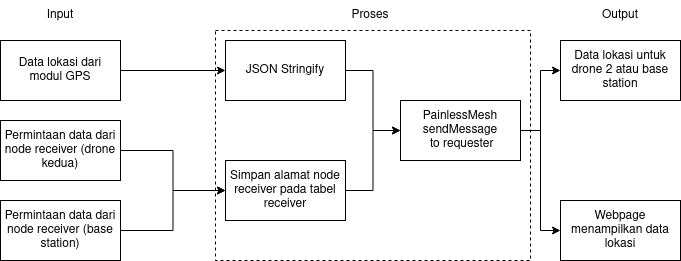
\includegraphics[scale=0.60]{./assets/IOProses}
	\caption{Desain konsep sistem}
\end{figure}
PainlessMesh bekerja menggunakan mode AP-STA pada mikrokontroler ESP32, dimana \textit{board} bekerja sebagai \textit{Wi-Fi Access Point} sekaligus \textit{Wi-Fi Station Mode} untuk membentuk sebuah jaringan mesh. Masing-masing node memiliki sebuah node ID, dan pada aplikasi penelitian ini memiliki penanda sebagai \textit{sender} (node yang mendata lokasi GPS dan mengirimkan data tersebut) dan \textit{receiver} (node yang menerima data lokasi tersebut).

\begin{figure}[h]
	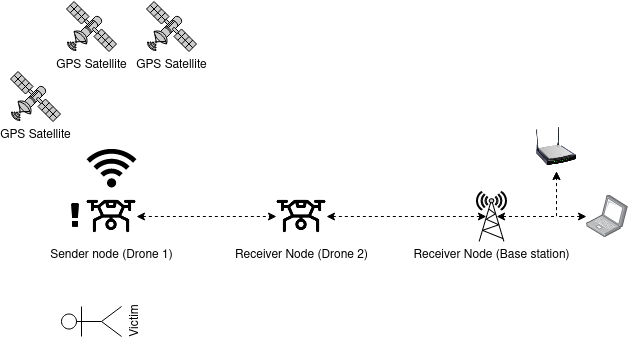
\includegraphics[scale=0.5]{./assets/Diagram Sistem}
	\caption{Diagram sistem}
\end{figure}

Node \textit{sender} memiliki modul GPS yang berkomunikasi dengan satelit untuk mendapatkan data lokasi yang terlampir dalam \textit{NMEA sentences}. Data tersebut kemudian diolah menggunakan \textit{library} TinyGPS++ untuk mengekstraksi data lokasi dari \textit{NMEA sentences} tersebut.

\textit{Sender node} memiliki sebuah \textit{flag} "locationReady" dimana jika nilainya \textit{"true"} maka dapat menerima permintaan data lokasi dari \textit{receiver node}. Kriteria untuk \textit{flag} tersebut memiliki nilai \textit{"true"} adalah telah mendapatkan \textit{lock} satelit minimal 3 dan telah mendapat nilai lintang dan bujur bukan nol.

Akses ke \textit{Base Station} menggunakan sebuah board ESP8266 yang terhubung secara serial dengan board ESP32 yang terhubung dengan jaringan mesh. Konfigurasi ini diperlukan karena limitasi dari board ESP32 yang memiliki koneksi bersamaan maksimum sebanyak 2 (1 dari klien \textit{Access Point}, 1 menjadi klien AP sebagai \textit{Station Mode}), sedangkan PainlessMesh menggunakan kedua mode tersebut untuk mempertahankan jaringan mesh yang dibentuk.

\section{Riset Terkait}
Terdapat beberapa penelitian yang telah dilaksanakan sebelumnya yang terkait dengan tugas akhir ini, yang akan digunakan sebagai dasar atau referensi dalam pengerjaan. Beberapa penelitian terkait dapat dilihat pada tabel 2.1.
\pagebreak
\begin{center}
	\footnotesize
	\captionof{table}{Penelitian terkait}
	\begin{longtable}{|p{0.5cm}|p{2cm}|p{2cm}|p{2cm}|p{2cm}|p{2cm}|}
		\hline
		&\textbf{Judul}&\textbf{Metode}&\textbf{Kesimpulan}&\textbf{Kelebihan}&\textbf{Kekurangan}\\
		\hline
		\cite{santosUseHighMobility2021}&Use of High Mobility Nodes to Improve Connectivity in Wireless Sensor Networks&PainlessMesh-based Opportunistic Mobile Ad Hoc Networks&Menggunakan high mobility nodes berupa drone sebagai messenger data antara cluster sensor dengan server&Penelitian mengimplementasikan metode security berbasis secret-key cryptography. Packet loss antara sensor dan server rendah, hanya 4,48\% pada kondisi terburuk walaupun packet melewati 2 hop.
		&Tidak menguji round-trip delay packet\\
		\hline
		\cite{chiaPerformanceEvaluationESP82662019a}&Performance Evaluation of ESP8266 Mesh Networks&Pengujian one-way delay dan data rate pada jaringan PainlessMesh ESP8266& Jumlah node berkorelasi dengan meningkatnya single hop delay dan menurunnya stabilitas jaringan, serta besar payload menentukan data rate dan korupsi data.&Penelitian menguji dari 2 hingga 16 node sehingga terlihat gambaran kasar stabilitas jaringan PainlessMesh. Kinerja jaringan 2 node memiliki delay 2.49 ms sehingga cukup untuk aplikasi yang tidak terlalu kompleks.&ESP8266 tidak memiliki performa yang cukup untuk mengirimkan dan menerima payload data yang besar. Pengujian data rate dibatasi pada 2 node. \\
		\hline
		\cite{manviImplementingWirelessMesh2020}&Implementing Wireless Mesh Network Topology Between Multiple Wi-Fi Powered Nodes for IoT Systems&Penggunaan 3 node PainlessMesh berbasis ESP32 untuk komunikasi multidirectional output sensor dan input push button&Mesh bersifat self-healing, pada saat terjadi disrupsi maka mesh secara otomatis mengatur diri.&Implementasi 3 node dan arah data bolak balik dapat dilakukan&Tidak ada pengujian jarak jauh\\
		\hline
		\cite{guoDustSensorMonitoring2021}&A dust sensor monitoring system using Wi-Fi mesh network&Implementasi 9 node berbasis ESP32 dan ESP-Mesh untuk monitoring tingkat debu pada suatu ruangan.&Sistem efektif dengan measurement error dibawah 5\%&Mesh dapat berfungsi tanpa intervensi manusia, memiliki sifat self-healing dan auto-configuration.& Jaringan memiliki topologi tree, bukan mesh murni, sehingga jika terjadi gangguan pada node akar maka proses self-heal berjalan lebih lama.\\
		\hline
	\end{longtable}
\end{center}
Berdasarkan penelitian yang telah dilakukan sebelumnya, maka penulis akan membatasi penelitian ke 3 node ESP32, menguji \textit{throughput, packet loss, round-trip delay,} dan \textit{signal strength (dBm)}; serta pengujian jarak antar node terhadap kinerja jaringan. Khusus untuk node base station akan disambungkan dengan sebuah board ESP8266 sebagai HTTP Server untuk koneksi web server yang menampilkan data lokasi dari node \textit{sender}.

\section{\textit{Unmanned Aerial Vehicles}}
UAV adalah sebuah pesawat terbang yang dapat mengudara tanpa awak \cite{lakshminarayananJointNetworkDisaster2015}, dikendalikan secara \textit{remote} atau secara otonom. Salah satu tipe UAV adalah \textit{quadcopter drone}. Pada sistem ini, UAV digunakan sebagai pengirim data lokasi GPS sebagai node \textit{sender}, dan penerima data lokasi GPS sebagai node \textit{receiver}.

\section{\textit{Quadcopter}}
Drone \textit{quadcopter} adalah suatu jenis UAV yang memiliki 4 rotor pada masing-masing sudut. Sama seperti helikopter, \textit{quadcopter} memiliki kemampuan untuk \textit{hover}. Terdapat sepasang rotor yang berputar searah jarum jam dan sepasang rotor yang berputar berlawanan arah jarum jam, sehingga pada kondisi \textit{steady state} total torsi pada \textit{drone} adalah nol. Hal tersebut juga menyebabkan konfigurasi \textit{quadcopter} tidak membutuhkan \textit{tail rotor}. Keempat rotor tersebut juga menghasilkan daya angkat yang besar, sehingga cocok digunakan untuk membawa \textit{payload}.

\section{ESP32}
Pada penelitian ini, ESP32 digunakan sebagai modul komunikasi antar node baik drone maupun base station. Board-board ESP32 dapat dikonfigurasikan menjadi jaringan mesh menggunakan mode APSTA/\textit{Coexistence Mode}, dimana secara bersamaan ESP32 mem-\textit{broadcast} SSID sambil terhubung dengan jaringan lain \cite{WiFiDriverESP32}. 

ESP32 juga mendukung protokol \textit{proprietary} buatan Espressif bernama 802.11 LR \textit{(Long Range)}, dengan jarak hingga 1 km selama ada \textit{line-of-sight} antara \textit{node}. \cite{WiFiDriverESP32}.
\begin{figure}[h]
	\centering
	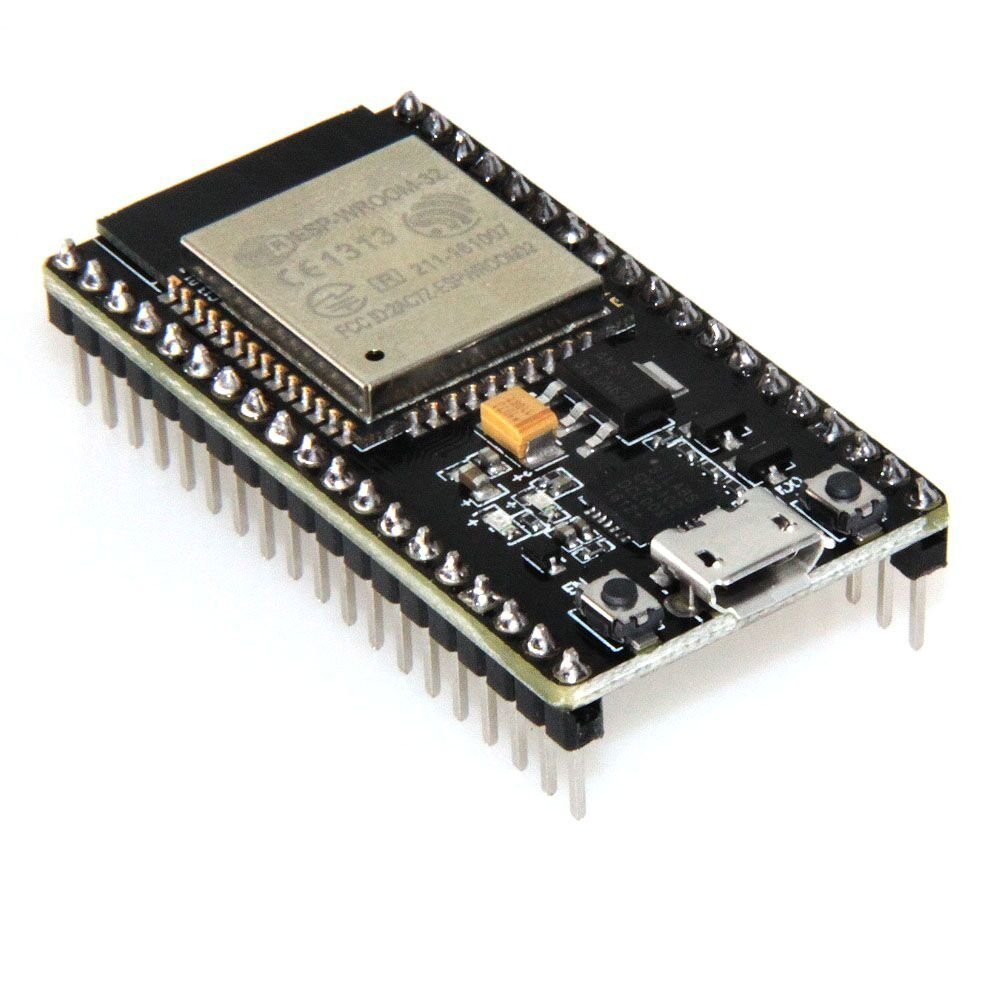
\includegraphics[scale=0.1]{./assets/ESP32}
	\caption{ESP32}
\end{figure}

\section{PainlessMesh}
PainlessMesh merupakan sebuah library yang memudahkan pengguna \textit{board} ESP32 dalam membuat sebuah jaringan mesh ad-hoc berbasis WiFi. Karena batasan dari \textit{board} ESP32, maka jaringan yang dihasilkan merupakan \textit{"pseudo-mesh"} atau mesh yang tidak sempurna, sehingga pada kondisi standar, semua node memiliki kedudukan yang sama dan diatur dalam topologi \textit{tree}.

Jaringan PainlessMesh menggunakan mode APSTA pada board ESP32, dimana setiap board ESP32, disebut dengan "node", berfungsi sebagai WiFi \textit{Access Point} (AP) sekaligus sebagai klien WiFi \textit{Station Mode}. Setiap node berbasis ESP32 dapat memiliki sebanyak 10 klien yang terhubung pada 1 AP, dan dapat terhubung pada AP lainnya sebagai sebuah klien.

\begin{figure}[h]
	\centering
	\includegraphics[scale=0.5]{./assets/painlessmesh}
	\caption{Topologi jaringan PainlessMesh \cite{HomeWikiPainlessMesh}, panah menunjukkan arah koneksi dari klien ke AP}
\end{figure}

Keistimewaan dari library PainlessMesh adalah kemampuannya untuk \textit{autoconfigure}, dimana setiap node dapat memutus sambungan dan menyambung ulang setiap saat, dan jaringan mesh dapat berjalan melalui proses konfigurasi secara otomatis.
% Daftar Pustaka
\selectlanguage{english}
\printbibliography[title={DAFTAR PUSTAKA}]

	
\end{document}